\documentclass[journal]{vgtc}                % final (journal style)
%\documentclass[review,journal]{vgtc}         % review (journal style)
%\documentclass[widereview]{vgtc}             % wide-spaced review
%\documentclass[preprint,journal]{vgtc}       % preprint (journal style)

%% Uncomment one of the lines above depending on where your paper is
%% in the conference process. ``review'' and ``widereview'' are for review
%% submission, ``preprint'' is for pre-publication, and the final version
%% doesn't use a specific qualifier.

%% Please use one of the ``review'' options in combination with the
%% assigned online id (see below) ONLY if your paper uses a double blind
%% review process. Some conferences, like IEEE Vis and InfoVis, have NOT
%% in the past.

%% Please note that the use of figures other than the optional teaser is not permitted on the first page
%% of the journal version.  Figures should begin on the second page and be
%% in CMYK or Grey scale format, otherwise, colour shifting may occur
%% during the printing process.  Papers submitted with figures other than the optional teaser on the
%% first page will be refused. Also, the teaser figure should only have the
%% width of the abstract as the template enforces it.

%% These few lines make a distinction between latex and pdflatex calls and they
%% bring in essential packages for graphics and font handling.
%% Note that due to the \DeclareGraphicsExtensions{} call it is no longer necessary
%% to provide the the path and extension of a graphics file:
%% 
\includegraphics{diamondrule} is completely sufficient.
%%
\ifpdf%                                % if we use pdflatex
  \pdfoutput=1\relax                   % create PDFs from pdfLaTeX
  \pdfcompresslevel=9                  % PDF Compression
  \pdfoptionpdfminorversion=7          % create PDF 1.7
  \ExecuteOptions{pdftex}
  \usepackage{graphicx}                % allow us to embed graphics files
  \DeclareGraphicsExtensions{.pdf,.png,.jpg,.jpeg} % for pdflatex we expect .pdf, .png, or .jpg files
\else%                                 % else we use pure latex
  \ExecuteOptions{dvips}
  \usepackage{graphicx}                % allow us to embed graphics files
  \DeclareGraphicsExtensions{.eps}     % for pure latex we expect eps files
\fi%

%% it is recomended to use ``\autoref{sec:bla}'' instead of ``Fig.~\ref{sec:bla}''
\graphicspath{{figures/}{pictures/}{images/}{./}} % where to search for the images

\usepackage{microtype}                 % use micro-typography (slightly more compact, better to read)
\PassOptionsToPackage{warn}{textcomp}  % to address font issues with \textrightarrow
\usepackage{textcomp}                  % use better special symbols
\usepackage{mathptmx}                  % use matching math font
\usepackage{times}                     % we use Times as the main font
\renewcommand*\ttdefault{txtt}         % a nicer typewriter font
\usepackage{cite}                      % needed to automatically sort the references
\usepackage{tabu}                      % only used for the table example
\usepackage{booktabs}                  % only used for the table example
%% We encourage the use of mathptmx for consistent usage of times font
%% throughout the proceedings. However, if you encounter conflicts
%% with other math-related packages, you may want to disable it.

%% In preprint mode you may define your own headline.
%\preprinttext{To appear in IEEE Transactions on Visualization and Computer Graphics.}

%% If you are submitting a paper to a conference for review with a double
%% blind reviewing process, please replace the value ``0'' below with your
%% OnlineID. Otherwise, you may safely leave it at ``0''.
\onlineid{0}

%% declare the category of your paper, only shown in review mode
\vgtccategory{Research}
%% please declare the paper type of your paper to help reviewers, only shown in review mode
%% choices:
%% * algorithm/technique
%% * application/design study
%% * evaluation
%% * system
%% * theory/model
\vgtcpapertype{please specify}

%% Paper title.
\title{NarVis: How to Explain An Advanced Visualization Design}

%% This is how authors are specified in the journal style

%% indicate IEEE Member or Student Member in form indicated below
\author{Roy G. Biv, Ed Grimley, \textit{Member, IEEE}, and Martha Stewart}
\authorfooter{
%% insert punctuation at end of each item
\item
 Roy G. Biv is with Starbucks Research. E-mail: roy.g.biv@aol.com.
\item
 Ed Grimley is with Grimley Widgets, Inc.. E-mail: ed.grimley@aol.com.
\item
 Martha Stewart is with Martha Stewart Enterprises at Microsoft
 Research. E-mail: martha.stewart@marthastewart.com.
}

%other entries to be set up for journal
\shortauthortitle{Biv \MakeLowercase{\textit{et al.}}: Global Illumination for Fun and Profit}
%\shortauthortitle{Firstauthor \MakeLowercase{\textit{et al.}}: Paper Title}

%% Abstract section.
\abstract{nothing here%
} % end of abstract

%% Keywords that describe your work. Will show as 'Index Terms' in journal
%% please capitalize first letter and insert punctuation after last keyword
\keywords{Radiosity, global illumination, constant time}

%% ACM Computing Classification System (CCS). 
%% See <http://www.acm.org/class/1998/> for details.
%% The ``\CCScat'' command takes four arguments.

\CCScatlist{ % not used in journal version
 \CCScat{K.6.1}{Management of Computing and Information Systems}%
{Project and People Management}{Life Cycle};
 \CCScat{K.7.m}{The Computing Profession}{Miscellaneous}{Ethics}
}

%% Uncomment below to include a teaser figure.
\teaser{
  \centering
  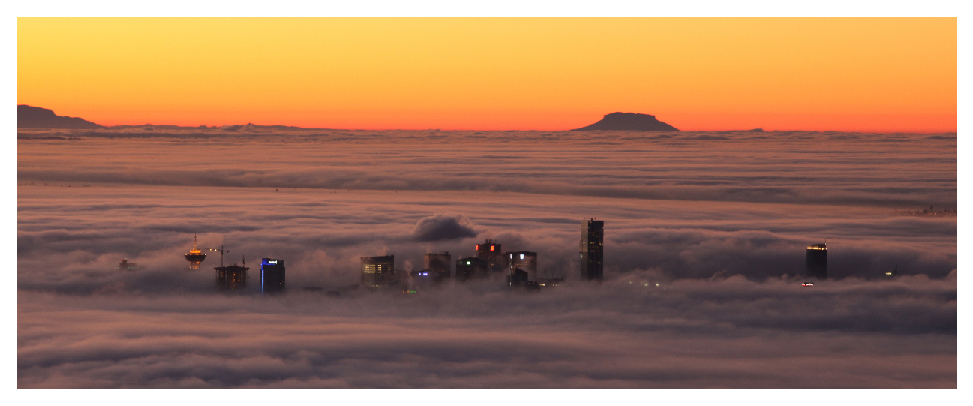
\includegraphics[width=\linewidth]{CypressView}
  \caption{In the Clouds: Vancouver from Cypress Mountain. Note that the teaser may not be wider than the abstract block.}
	\label{fig:teaser}
}

%% Uncomment below to disable the manuscript note
%\renewcommand{\manuscriptnotetxt}{}

%% Copyright space is enabled by default as required by guidelines.
%% It is disabled by the 'review' option or via the following command:
% \nocopyrightspace

\vgtcinsertpkg

%%%%%%%%%%%%%%%%%%%%%%%%%%%%%%%%%%%%%%%%%%%%%%%%%%%%%%%%%%%%%%%%
%%%%%%%%%%%%%%%%%%%%%% START OF THE PAPER %%%%%%%%%%%%%%%%%%%%%%
%%%%%%%%%%%%%%%%%%%%%%%%%%%%%%%%%%%%%%%%%%%%%%%%%%%%%%%%%%%%%%%%%

\begin{document}

%% The ``\maketitle'' command must be the first command after the
%% ``\begin{document}'' command. It prepares and prints the title block.

%% the only exception to this rule is the \firstsection command
\maketitle

\section{Introduction} %for journal use above \firstsection{..} instead
Advanced visualization techniques are effective for data analysis[][]. By introducing metaphors borrowed from nature \cite{cao_whisper:_2012,huron_visual_2013}, applying carefully designed layout algorithms\cite{wu_opinionflow:_2014,chi_morphable_2015}, and sophisticatedly combining existing visualizations\cite{zhao_x0023;fluxflow:_2014}, novel visual presentations help people identify patterns, trends and correlations hidden in data. However, these advanced visualizations are usually not intuitively recognizable. Users need to go through some training, for example, reading a long and boring literal description, before they grasp the knowledge required to understand and freely explore a visualization.\par
What is more, even designers of these advanced visualizations suffer when they are required to introduce their design, especially when the visual encoding has complicated logic dependency, or when their audience have little prior knowledge about visualization techniques.\par
As a result, these advanced visualization technologies, in spite of
the fact that their utility has been verified by domain experts from various fields, gain little exposure outside the visual community. Unaware of or unable to understand these advanced visualizations, main stream media is still dominated by naïve visualizations, such as bar charts, pie charts and so on. \par
For a visualization, its design space can be described as the orthogonal combination of two aspects: graphical elements called marks and visual channels to control their appearance\cite{munzner_visualization_2014}. But why the explanation of these two things is so complicated? \par
This problem mainly arises from the great amount of information that an advanced visualization design attempts to deliver with visual encoding. First, it would overload an audience if we inundated them with all the information at one time. Second, even if we tried to explain it sequentially, considering the logic dependency existing among visual elements, an improper explanation could totally confuse the audience. For example, the topic streams of a theme river should be explained before the keywords mapping on them, otherwise, the audience would get totally lost. Third, when digesting such a considerable amount of information, audiences can easily get distracted or forget previous information.  [ ]. \par
Thus, a specific order of encoding explanation becomes necessary. Attention guidance and reminders are also needed to make sure that audiences are following order, not getting distracted or forgetting previous information.\par
Narrative, which means “connected events presented in a sequence”, has long been used to share complex information. As the data visualization field is maturing, many researchers have moved their focus from analysis to presentation, making narrative data visualization an emerging topic\cite{kosara_storytelling:_2013}. Many efforts have been
made to define, classify, and provide design suggestions for narrative data visualization\cite{segel_narrative_2010,hullman_deeper_2013,gershon_what_2001}. Some visualization systems have already incorporated narrative modules into their design\cite{eccles_stories_2007,bryan_temporal_2016}. However, current work is mainly focused on communicating the conclusion of analyses, rather than guiding the audience how to read a visualization. \par
Here, we present a prototype to adopt narrative techniques to create a visual encoding explanation. Based on our analysis of the structure, logic dependency, and visual distraction existing in a visualization design, we develop an authoring tool to decompose a visualization, reorganize extracted visual elements, and explain their visual encodings one by one through animated transition in the form of slideshow. Through incorporating a narrative sequence, appropriate chunks of information, rather than all the information, is delivered to the audience at one time, effectively avoiding information overload. Reminders, such as questions, summarizations and repetitions are woven into the narrative sequence to enhance the audience’s memory while visual attention guidance, such as flickering, highlighting, and morphing are used to lead their attention to newly added information. (字数超了就删掉)\par
To the best of our knowledge, this is the first attempt to explain visual encoding with narrative. We believe we make the following contributions: 1). Analysis of the structure, logic dependency, and visual distraction which exists in a visualization design. 2) A framework for explaining narrative visual encoding. 3) An authoring tool to generate and edit the narrative visual encoding explanation
 We conjecture our work can motivate and enable people to use more advanced visualization designs.\par
\section {Related work}
In this section, we provide an overview of prior research around the analysis of narrative structure in data visualization, animation in data visualization, and existing authoring tools for narrative visualizations.\par
\subsection{Structure of Narrative Data Visualization}
Narrative is as old as human history. [cite something] People in the fields of literature, comics \cite{cohn_visual_2013} and cinema \cite{schmidt_living_2017} have gone to great lengths to analyse the sequencing and forms of grouping used in a narrative, as well as how they affect the meaning a narrative tries to deliver. \par
Some people believe that work from other fields can inspire researchers in the visual data community. Amini et al\cite{amini_understanding_2015} borrowed concepts from comics \cite{cohn_visual_2013} to classify and analyse the structure of data videos. Wang et al \cite{wang_animated_2016} adopt two representative tactics, time-remapping and foreshadowing, from cinematographers to organize a narrative sequence for visualizing temporal data. \par
Other researchers, on the other side, focus on the narrative structures exclusively for data visualization. \par
Satyanarayan and Heer, through interviews with professional journalists\cite{satyanarayan_authoring_2014} define the core abstractions of narrative data visualization as state-based scenes, visualization parameters, dynamic graphical and textual annotations, and interaction triggers. Hullman et al\cite{hullman_deeper_2013}, by identifying the change in data attributes, propose a graph-driven approach to automatically identify effective narrative sequences for linearly presenting a set of visualizations. \par
These works, however, rarely discuss the narrative structures used for visual encoding scheme, which is fundamental to a visualization. We hope our work can fill this gap.\par
\subsection{Animation for data visualization}
There is a wide discussion about the effects of animation when used in a data visualization environment.\par 
Animation can facilitate the cognitive process. Heer and Robertson \cite{heer_animated_2007-1} confirmed the effectiveness of animation when relating data visualizations backed by a shared dataset. Ruchikachorn et al\cite{ruchikachorn_learning_2015}, going a step further, design morphing animations which bridge the gap between a familiar visualization and an unfamiliar one, thus introducing a new visualization design through animation. Graphdiaries \cite{bach_graphdiaries:_2014} use animation to help audiences track and understand changes in a dynamic visualization. \par
On the other hand, animation can be an effective tool to attract and guide visual attention. Huber et al \cite{huber_visualizing_2005} study the perceptual properties of different kinds of animation, as well as their effects on human attention. Waldner et al \cite{waldner_attractive_2014} focused on a specific animation: flicker. By dividing the animation into an “orientation stage” and an “engagement stage”, they strike a good balance between the attraction effectiveness and annoyance caused by flickering. \par
It is, however, noteworthy that animation, in spite of all the advantages mentioned above, can bring about negative effects when used improperly\cite{robertson_effectiveness_2008}. Our work is based on the results of these researches, which give us a guideline on how to implement animations in our system.\par
\subsection{Authoring tools for narrative visualization}
The extensive needs of data communication exist not only in the data visualization field but also in journalism, media, and so on. This has motivated researchers to investigate ways for authoring narrative visualization. \par
User experience is of great concern when utilising an authoring tool. Sketch story \cite{lee_sketchstory:_2013}, with its freeform sketch interaction, provides a more engaging way to create and present narrative visualization. Dataclips \cite{amini_authoring_2017}lower the barrier of crafting narrative visualization by providing a library of data clips, allowing non-experts to be involved in the production of narrative visualization. \par
However, it is the information delivery that is the core consideration of an authoring tool. Existing authoring tools usually choose a specific type of narrative visualization based on the information they want to convey.\cite{amini_authoring_2017}Meanwhile, integrating an authoring tool for narrative visualization with a  data analysis tool has become a trend since it effectively bridges the gap between data analysis and data communication. \cite{eccles_stories_2007,bryan_temporal_2016,lee_more_2015}\par 
These tools offer inspiring user interaction design as well as good examples to implement narrative visualization. However, they treat visual encodings as cognitively obvious attributes that can be universally and immediately recognized without a formal introduction, making them inapplicable for our purpose. \par
\section{}
\section{Bibliography Instructions}

\begin{itemize}
\item Sort all bibliographic entries alphabetically but the last name of the first author. This \LaTeX/bib\TeX\ template takes care of this sorting automatically.
\item Merge multiple references into one; e.\,g., use \cite{Max:1995:OMF,Kitware:2003} (not \cite{Kitware:2003}\cite{Max:1995:OMF}). Within each set of multiple references, the references should be sorted in ascending order. This \LaTeX/bib\TeX\ template takes care of both the merging and the sorting automatically.
\item Verify all data obtained from digital libraries, even ACM's DL and IEEE Xplore  etc.\ are sometimes wrong or incomplete.
\item Do not trust bibliographic data from other services such as Mendeley.com, Google Scholar, or similar; these are even more likely to be incorrect or incomplete.
\item Articles in journal---items to include:
  \begin{itemize}
  \item author names
	\item title
	\item journal name
	\item year
	\item volume
	\item number
	\item month of publication as variable name (i.\,e., \{jan\} for January, etc.; month ranges using \{jan \#\{/\}\# feb\} or \{jan \#\{-{}-\}\# feb\})
  \end{itemize}
\item use journal names in proper style: correct: ``IEEE Transactions on Visualization and Computer Graphics'', incorrect: ``Visualization and Computer Graphics, IEEE Transactions on''
\item Papers in proceedings---items to include:
  \begin{itemize}
  \item author names
	\item title
	\item abbreviated proceedings name: e.\,g., ``Proc.\textbackslash{} CONF\_ACRONYNM'' without the year; example: ``Proc.\textbackslash{} CHI'', ``Proc.\textbackslash{} 3DUI'', ``Proc.\textbackslash{} Eurographics'', ``Proc.\textbackslash{} EuroVis''
	\item year
	\item publisher
	\item town with country of publisher (the town can be abbreviated for well-known towns such as New York or Berlin)
  \end{itemize}
\item article/paper title convention: refrain from using curly brackets, except for acronyms/proper names/words following dashes/question marks etc.; example:
\begin{itemize}
	\item paper ``Marching Cubes: A High Resolution 3D Surface Construction Algorithm''
	\item should be entered as ``\{M\}arching \{C\}ubes: A High Resolution \{3D\} Surface Construction Algorithm'' or  ``\{M\}arching \{C\}ubes: A high resolution \{3D\} surface construction algorithm''
	\item will be typeset as ``Marching Cubes: A high resolution 3D surface construction algorithm''
\end{itemize}
\item for all entries
\begin{itemize}
	\item DOI can be entered in the DOI field as plain DOI number or as DOI url; alternative: a url in the URL field
	\item provide full page ranges AA-{}-BB
\end{itemize}
\item when citing references, do not use the reference as a sentence object; e.\,g., wrong: ``In \cite{Lorensen:1987:MCA} the authors describe \dots'', correct: ``Lorensen and Cline \cite{Lorensen:1987:MCA} describe \dots''
\end{itemize}

\section{Example Section}

Lorem ipsum dolor sit amet, consetetur sadipscing elitr, sed diam
nonumy eirmod tempor invidunt ut labore et dolore magna aliquyam erat,
sed diam voluptua. At vero eos et accusam et justo duo dolores et ea
rebum. Stet clita kasd gubergren, no sea takimata sanctus est Lorem
ipsum dolor sit amet. Lorem ipsum dolor sit amet, consetetur
sadipscing elitr, sed diam nonumy eirmod tempor invidunt ut labore et
dolore magna aliquyam erat, sed diam
voluptua~\cite{Kitware:2003,Max:1995:OMF}. At vero eos et accusam et
justo duo dolores et ea rebum. Stet clita kasd gubergren, no sea
takimata sanctus est Lorem ipsum dolor sit amet. Lorem ipsum dolor sit
amet, consetetur sadipscing elitr, sed diam nonumy eirmod tempor
invidunt ut labore et dolore magna aliquyam erat, sed diam
voluptua. At vero eos et accusam et justo duo dolores et ea
rebum. Stet clita kasd gubergren, no sea takimata sanctus est.

\section{Exposition}

Duis autem vel eum iriure dolor in hendrerit in vulputate velit esse
molestie consequat, vel illum dolore eu feugiat nulla facilisis at
vero eros et accumsan et iusto odio dignissim qui blandit praesent
luptatum zzril delenit augue duis dolore te feugait nulla
facilisi. Lorem ipsum dolor sit amet, consectetuer adipiscing elit,
sed diam nonummy nibh euismod tincidunt ut laoreet dolore magna
aliquam erat volutpat~\cite{Kindlmann:1999:SAG}.

\begin{equation}
\sum_{j=1}^{z} j = \frac{z(z+1)}{2}
\end{equation}

Lorem ipsum dolor sit amet, consetetur sadipscing elitr, sed diam
nonumy eirmod tempor invidunt ut labore et dolore magna aliquyam erat,
sed diam voluptua. At vero eos et accusam et justo duo dolores et ea
rebum. Stet clita kasd gubergren, no sea takimata sanctus est Lorem
ipsum dolor sit amet. Lorem ipsum dolor sit amet, consetetur
sadipscing elitr, sed diam nonumy eirmod tempor invidunt ut labore et
dolore magna aliquyam erat, sed diam voluptua. At vero eos et accusam
et justo duo dolores et ea rebum. Stet clita kasd gubergren, no sea
takimata sanctus est Lorem ipsum dolor sit amet.

\subsection{Lorem ipsum}

Lorem ipsum dolor sit amet (see \autoref{tab:vis_papers}), consetetur sadipscing elitr, sed diam
nonumy eirmod tempor invidunt ut labore et dolore magna aliquyam erat,
sed diam voluptua. At vero eos et accusam et justo duo dolores et ea
rebum. Stet clita kasd gubergren, no sea takimata sanctus est Lorem
ipsum dolor sit amet. Lorem ipsum dolor sit amet, consetetur
sadipscing elitr, sed diam nonumy eirmod tempor invidunt ut labore et
dolore magna aliquyam erat, sed diam voluptua. At vero eos et accusam
et justo duo dolores et ea rebum. Stet clita kasd gubergren, no sea
takimata sanctus est Lorem ipsum dolor sit amet. Lorem ipsum dolor sit
amet, consetetur sadipscing elitr, sed diam nonumy eirmod tempor
invidunt ut labore et dolore magna aliquyam erat, sed diam
voluptua. At vero eos et accusam et justo duo dolores et ea
rebum. 

\begin{table}[tb]
  \caption{VIS/VisWeek accepted/presented papers: 1990--2015.}
  \label{tab:vis_papers}
  \scriptsize%
	\centering%
  \begin{tabu}{%
	r%
	*{7}{c}%
	*{2}{r}%
	}
  \toprule
   year & \rotatebox{90}{Vis/SciVis} &   \rotatebox{90}{SciVis conf} &   \rotatebox{90}{InfoVis} &   \rotatebox{90}{VAST} &   \rotatebox{90}{VAST conf} &   \rotatebox{90}{TVCG @ VIS} &   \rotatebox{90}{CG\&A @ VIS} &   \rotatebox{90}{VIS/VisWeek} \rotatebox{90}{incl. TVCG/CG\&A}   &   \rotatebox{90}{VIS/VisWeek} \rotatebox{90}{w/o TVCG/CG\&A}   \\
  \midrule
  2015 & 33 & 9 & 38 & 33 & 14 & 17 & 15 & 159 & 127 \\
  2014 & 34 &   & 45 & 33 & 21 & 20 &   & 153 & 133 \\
  2013 & 31 &   & 38 & 32 &   & 20 &   & 121 & 101 \\
  2012 & 42 &   & 44 & 30 &   & 23 &   & 139 & 116 \\
  2011 & 49 &   & 44 & 26 &   & 20 &   & 139 & 119 \\
  2010 & 48 &   & 35 & 26 &   &   &   & 109 & 109 \\
  2009 & 54 &   & 37 & 26 &   &   &   & 117 & 117 \\
  2008 & 50 &   & 28 & 21 &   &   &   & 99 & 99 \\
  2007 & 56 &   & 27 & 24 &   &   &   & 107 & 107 \\
  2006 & 63 &   & 24 & 26 &   &   &   & 113 & 113 \\
  2005 & 88 &   & 31 &   &   &   &   & 119 & 119 \\
  2004 & 70 &   & 27 &   &   &   &   & 97 & 97 \\
  2003 & 74 &   & 29 &   &   &   &   & 103 & 103 \\
  2002 & 78 &   & 23 &   &   &   &   & 101 & 101 \\
  2001 & 74 &   & 22 &   &   &   &   & 96 & 96 \\
  2000 & 73 &   & 20 &   &   &   &   & 93 & 93 \\
  1999 & 69 &   & 19 &   &   &   &   & 88 & 88 \\
  1998 & 72 &   & 18 &   &   &   &   & 90 & 90 \\
  1997 & 72 &   & 16 &   &   &   &   & 88 & 88 \\
  1996 & 65 &   & 12 &   &   &   &   & 77 & 77 \\
  1995 & 56 &   & 18 &   &   &   &   & 74 & 74 \\
  1994 & 53 &   &   &   &   &   &   & 53 & 53 \\
  1993 & 55 &   &   &   &   &   &   & 55 & 55 \\
  1992 & 53 &   &   &   &   &   &   & 53 & 53 \\
  1991 & 50 &   &   &   &   &   &   & 50 & 50 \\
  1990 & 53 &   &   &   &   &   &   & 53 & 53 \\
  \midrule
  \textbf{sum} & \textbf{1515} & \textbf{9} & \textbf{595} & \textbf{277} & \textbf{35} & \textbf{100} & \textbf{15} & \textbf{2546} & \textbf{2431} \\
  \bottomrule
  \end{tabu}%
\end{table}

\subsection{Mezcal Head}

Lorem ipsum dolor sit amet (see \autoref{fig:sample}), consetetur sadipscing elitr, sed diam
nonumy eirmod tempor invidunt ut labore et dolore magna aliquyam erat,
sed diam voluptua. At vero eos et accusam et justo duo dolores et ea
rebum. Stet clita kasd gubergren, no sea takimata sanctus est Lorem
ipsum dolor sit amet. Lorem ipsum dolor sit amet, consetetur
sadipscing elitr, sed diam nonumy eirmod tempor invidunt ut labore et
dolore magna aliquyam erat, sed diam voluptua. At vero eos et accusam
et justo duo dolores et ea rebum. Stet clita kasd gubergren, no sea
takimata sanctus est Lorem ipsum dolor sit amet. 

\subsubsection{Duis Autem}

Lorem ipsum dolor sit amet, consetetur sadipscing elitr, sed diam
nonumy eirmod tempor invidunt ut labore et dolore magna aliquyam erat,
sed diam voluptua. At vero eos et accusam et justo duo dolores et ea
rebum. Stet clita kasd gubergren, no sea takimata sanctus est Lorem
ipsum dolor sit amet. Lorem ipsum dolor sit amet, consetetur
sadipscing elitr, sed diam nonumy eirmod tempor invidunt ut labore et
dolore magna aliquyam erat, sed diam voluptua. At vero eos et accusam
et justo duo dolores et ea rebum. Stet clita kasd gubergren, no sea
takimata sanctus est Lorem ipsum dolor sit amet. Lorem ipsum dolor sit
amet, consetetur sadipscing elitr, sed diam nonumy eirmod tempor
invidunt ut labore et dolore magna aliquyam erat, sed diam
voluptua. At vero eos et accusam et justo duo dolores et ea
rebum. Stet clita kasd gubergren, no sea takimata sanctus est. Lorem
ipsum dolor sit amet.

\begin{figure}[tb]
 \centering % avoid the use of \begin{center}...\end{center} and use \centering instead (more compact)
 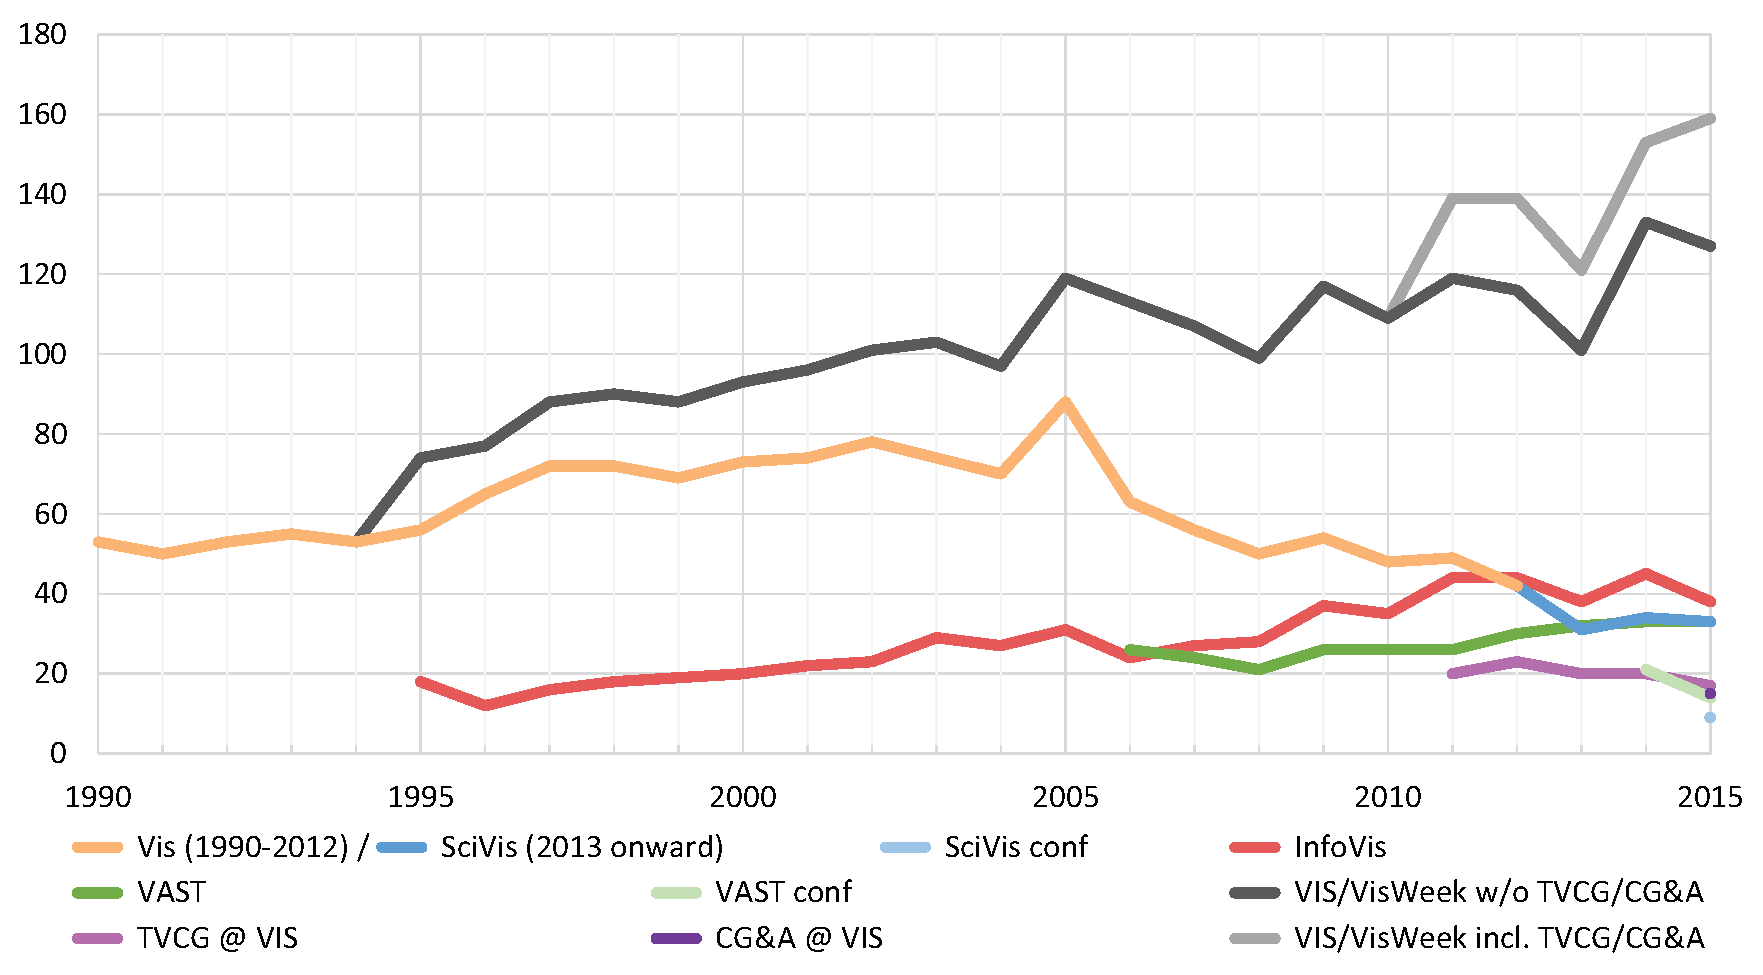
\includegraphics[width=\columnwidth]{paper-count-w-2015-new}
 \caption{A visualization of the data from \autoref{tab:vis_papers}. The image is from \cite{Isenberg:2017:VMC} and is in the public domain.}
 \label{fig:sample}
\end{figure}

\subsubsection{Ejector Seat Reservation}

Duis autem~\cite{Lorensen:1987:MCA}\footnote{The algorithm behind
Marching Cubes \cite{Lorensen:1987:MCA} had already been
described by Wyvill et al. \cite{Wyvill:1986:DSS} a year
earlier.} vel eum iriure dolor in hendrerit
in vulputate velit esse molestie consequat,\footnote{Footnotes
appear at the bottom of the column.} vel illum dolore eu
feugiat nulla facilisis at vero eros et accumsan et iusto odio
dignissim qui blandit praesent luptatum zzril delenit augue duis
dolore te feugait nulla facilisi. Lorem ipsum dolor sit amet,
consectetuer adipiscing elit, sed diam nonummy nibh euismod tincidunt
ut laoreet dolore magna aliquam erat volutpat.


\paragraph{Confirmed Ejector Seat Reservation}

Ut wisi enim ad minim veniam, quis nostrud exerci tation ullamcorper
suscipit lobortis nisl ut aliquip ex ea commodo
consequat~\cite{Nielson:1991:TAD}. Duis autem vel eum iriure dolor in
hendrerit in vulputate velit esse molestie consequat, vel illum dolore
eu feugiat nulla facilisis at vero eros et accumsan et iusto odio
dignissim qui blandit praesent luptatum zzril delenit augue duis
dolore te feugait nulla facilisi.

\paragraph{Rejected Ejector Seat Reservation}

Ut wisi enim ad minim veniam, quis nostrud exerci tation ullamcorper
suscipit lobortis nisl ut aliquip ex ea commodo consequat. Duis autem
vel eum iriure dolor in hendrerit in vulputate velit esse molestie


\section{Conclusion}
\cite{isenberg_visualization_2017}
Lorem ipsum dolor sit amet, consetetur sadipscing elitr, sed diam
nonumy eirmod tempor invidunt ut labore et dolore magna aliquyam erat,
sed diam voluptua. At vero eos et accusam et justo duo dolores et ea
rebum. Stet clita kasd gubergren, no sea takimata sanctus est Lorem
ipsum dolor sit amet. Lorem ipsum dolor sit amet, consetetur
sadipscing elitr, sed diam nonumy eirmod tempor invidunt ut labore et
dolore magna aliquyam erat, sed diam voluptua. At vero eos et accusam
et justo duo dolores et ea rebum. Stet clita kasd gubergren, no sea
takimata sanctus est Lorem ipsum dolor sit amet. Lorem ipsum dolor sit
amet, consetetur sadipscing elitr, sed diam nonumy eirmod tempor
invidunt ut labore et dolore magna aliquyam erat, sed diam
voluptua. At vero eos et accusam et justo duo dolores et ea
rebum.
\cite{borkin_what_2013,dunne_rapid_2012}

%% if specified like this the section will be committed in review mode
\acknowledgments{
The authors wish to thank A, B, C. This work was supported in part by
a grant from XYZ.}

%\bibliographystyle{abbrv}
\bibliographystyle{abbrv-doi}
%\bibliographystyle{abbrv-doi-narrow}
%\bibliographystyle{abbrv-doi-hyperref}
%\bibliographystyle{abbrv-doi-hyperref-narrow}

\bibliography{template,ref}
\end{document}

